\chapter{基本的な使い方}
%\label{chap:chapter1}
chapter, section, subsectionや図の挿入、文献引用などのやり方は、本章のソースファイル(chapter1.tex, reference.bib)と出力されたpdfファイルを見比べればわかる。
\section{文献引用の仕方}
このテンプレートでは、BibTeXを使えるようにしている。

また、文献リストのフォーマットは、\url{https://yosuke-nakata.net/blog}からダウンロードした"apsrev4-2ja.bst"というbibtexスタイルファイルを使用している。
これは、アメリカ物理学会(APS)の標準のbibtexスタイルファイル"apsrev4-2.bst"を改造して、日本語の本も表示できるようにしたものらしい。
\subsection{BibTeXの使い方}
文献の引用は、例えば\cite{Okuda2013a}のように行う(ソースファイルchapter1.tex参照)。
reference.bibのファイルに文献リストを登録しておけば、
このようにするだけで、自動的に文献リストが作成される。

reference.bibファイルに入力する内容は、Google Scholarなどから引っ張ってくる。
Google Scholarで引用のマーク(図\ref{fig:googleScholar})をクリックすると、
図\ref{fig:quote}のようなものが出てくる。
次に、BibTeXをクリックすると、図\ref{fig:bibtex}のようなテキストが出てくる。
これをreference.bibにコピペする(ただし、Google Scholarのcitationはたまにおかしいのが出てくるので、信用し過ぎない方がいい。論文誌のウェブページからもbibtex用のcitationの情報はダウンロードできることがあり、その方が信用できる)。

\begin{figure}[htbp]
	\centering
	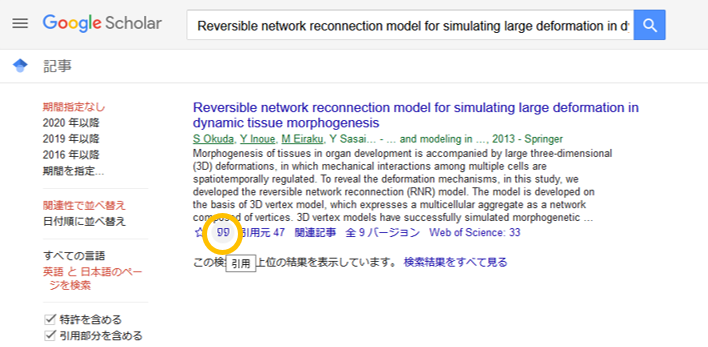
\includegraphics[width=12cm,clip]{fig/googleScholar.png}
	\caption{Google Scholarでの検索結果。引用のマークをクリックする。}
	\label{fig:googleScholar}
\end{figure}

\begin{figure}[htbp]
	\centering
	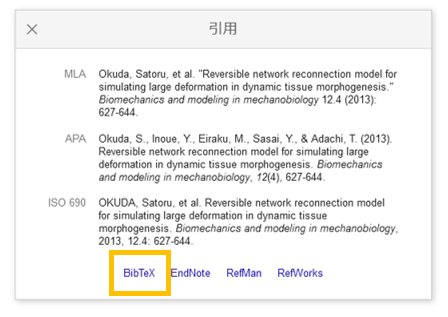
\includegraphics[width=10cm,clip]{fig/quote.png}
	\caption{引用のポップアップ。BibTeXをクリックする。}
	\label{fig:quote}
\end{figure}

% main.texで定義したclearpagefigure環境を使う場合は、
\begin{clearpagefigure}%[htbp]
	%\centering
	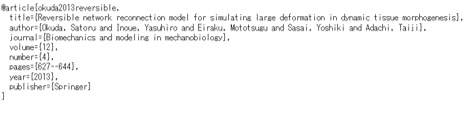
\includegraphics[width=12cm,clip]{fig/bibtex.png}
	\caption{BibTeX. これを.bibファイルにコピペする。}
	\label{fig:bibtex}
\end{clearpagefigure}
